\chapter{GPU Programming}

Increase of processors performance has been for a long time driven by Moore's law -- \enquote{The complexity for minimum component costs has increased at a rate of roughly a factor of two per year. Certainly over the short term this rate can be expected to continue, if not to increase. Over the longer term, the rate of increase is a bit more uncertain, although there is no reason to believe it will not remain constant for at least 10 years} \citep{MooresLaw}. This \enquote{law}, if we may call it that way, is unfortunately limited by physical properties of components used within modern processors. These limits are both on the side of possible processing speed, and on the side of size and number of transistors in the processor core. Over the last years, scientists are predicting end of Moore's law \citep{MooresLawEnd}, and their voices are louder, since the size of transistors in the \acrfull{acc:cpu} reached $7nm$ in 2018 \citep{SamsungSevenNm}. 

Processors manufactures are well aware of the physical complications arising from the small size of the transistors, and invest more effort into multi--core processors. These processors have a number of independent cores, that can be utilized in parallel and can possibly increase the performance of the processor linearly in respect to the number of cores. To name a few, last server processors by Intel\textsuperscript{\textregistered} Xeon\textsuperscript{\textregistered} Platinum 8380 Processor with 40 cores and 80 threads \citep{IntelXeonPlatinum}, as well as AMD EPYC\texttrademark\ 7763 with 64 cores and 128 threads \citep{AMDEpyc}, are great example.

\acrfullpl{acc:gpu} takes this idea of multi--cores processors further. Rather than increasing single--thread performance, the \gpu manufactures are focusing on massive parallelism using a great number of cores working in highly parallel and distributed manner \citep{GPUComputingOwens}. Using this approach, the \gpu programming offer promising performance. Common consumer \acrshortpl{acc:gpu} can easily outperform current high--end \acrshortpl{acc:cpu} in the instruction throughput and memory bandwidth. These demands originally came from the game industry, which place great emphasis on parallel processing and reasonably real--time latency. 

Decision about the architecture however influence the way \gpu are programmed. Unlike \cpu, which is can run generic code, \gpu is suited for specific kind of algorithms, that can fully use the underlying hardware. The program needs to have following mandatory properties to make it possible to run on \gpu \citep{GPUComputingOwens}:
\begin{itemize}
    \item \textit{Large computation demands} -- \gpu can deliver enormous performance, but has weak performance for short tasks without a lot of data. The overhead of allocating memory on \gpu and moving it between can easily outweigh the advantage of using it. On the other hand, the real--time rendering require hundreds of operations per pixel, and \gpu can easily meet these demands.
    \item \textit{Significant parallelism} -- the algorithm needs to be easy to parallelize and ideally scale to as many cores as possible. Whereas \cpu provides tens of cores (up to 64 today), the \gpu have hundreds or thousands of them (current cutting-edge \gpu designed especially for \acrshort{acc:ai}, NVIDIA V100, has 5120 CUDA cores \citep{nvidiav100spec}), although with smaller per--core performance. If can algorithm utilize only a few of them, it may be slower than on multi--core \cpu. Once again, real--time rendering can render each pixel independently, which makes it perfect candidate for \gpu computing.
    \item \textit{Throughput over latency} -- because the \gpu is highly parallel, the throughput is more important than the absolute latency of individual operations. From the point of rendering, human eye can perceive pictures in order of milliseconds. Operations in modern processors take in order of nanoseconds. Therefore, the absolute time to render a single pixel is not important as long as all the pixels are rendered in the same order of time. The algorithms cannot make assumptions about the running time of individual parts, but rather on the running time of the task as a whole.
\end{itemize}

\acrlong{acc:ea} fits well into these categories, as the individuals' fitness evaluation may be processed in parallel and independently. The crossover and mutation operators may be parallelized as well, as they operate and individuals or small set of individuals. We may parallelize the algorithm even more by processing each gene separately, as presented by \citet{CHENG2019514}.


%%%%%%%%%%%%%%%
%%           %%
%%  HISTORY  %%
%%           %%
%%%%%%%%%%%%%%%
\section{History}

Historically, \gpu come from needs of game industry for real--time rendering. In the rendering process, a list of geometric primitives, usually triangle, are processed through number of stages to form a final picture. The primitives can be processed independently and therefore in parallel, which makes real--time rendering the ideal case for use of \gpu. The typical operations in graphics consists of \citep{GPUComputingOwens}\index{rendering pipeline}:
\begin{itemize}
    \item Vertex stage, that transforms and compute properties per vertex. Typical operations are transformation of the geometric primitives from world space (that is the coordinates in the scene) into screen space (that is the coordinates in respect to the viewer point of view) and computing additional vertex properties like texture coordinates.
    \item Primitive assembly, that transform geometric primitives into triangles -- the standard geometric primitive for \gpu to understand. This stage may also clip the primitives, that are not in the view of the observer and save some computation in the following stages.
    \item Rasterization takes generated triangles and determine, which pixels correspond to provided triangle. These pixels do not necessary need match number of pixels of the screen and are usually referred as fragments (for example superscaling technique renders picture in higher resolution and then downsample the final picture to match screen resolution \citep{GameGraphicProgramming}). Each triangle may be composed by hundreds or thousands of fragments. Moreover, the rasterization typically interpolate vertex properties between the fragments.
    \item Fragment stage process each fragment and typically determine the final color of the fragment. It may compute fragment interactions with the lights in the scene, fetch colors from textures and so on. This stage is usually most demanding, as typical scene consists of millions of fragments.
    \item Composition stage assembles all the fragments into a final image. It may among other test fragments visibility and their blending.
\end{itemize}

The stages \gpu performs is usually referred as \emph{rendering pipeline} and may slightly differ. At the beginning, stages mentioned above have been preprogrammed by the manufacture and developers have only a limited options how to influence the stages of the pipeline (also known as the fixed--function pipeline). As the software complexity increased, the need for more control arise and the manufactures provided way to program the individual stages of the pipeline. These programs are called \emph{shaders} and their capabilities improved over the years. In 2006, Microsoft introduce Shading Model 4.0, which allowed using same programming interface and hardware both for vertex and fragment shader \citep{DirectX10}. Not only that, but more stages emerged (like tessellation and geometry shaders) to allow developers more control. Today, two major \acrfull{acc:api} exists -- proprietary  DirectX and open--source OpenGL. Note that some operations of the rendering pipeline, such as primitive assembly, rasterization, and composition are still implemented by the \gpu manufactures and in most cases are implemented by special--purpose hardware components \citep{SoftwareRasterization}. They are therefore integral part of the rendering pipeline and are not possible to modify.

Soon, scientists and engineers identified many more problems suitable for processing on \gpu. Although some parts of the rendering pipeline were fully programmable, the pipeline still inherently graphical and some stages are not possible to skip. To run general--purpose programs on \gpu required encoding the problem in the domain of geometric primitives and use available programmable and special--purpose hardware to implement the algorithm. Moreover, the programmers need to decide which part of the hardware will execute which part of the calculation and how the pipeline's fixed stages will affect the data structure. As shader programs do not have access to shared memory, the data passing were realized using textures, vertices, and fragment properties \citep{GPUComputingOwens}. These complications discouraged general use of \gpu for general--purpose programs, although some efforts have been made to hide underlying rendering pipeline from the programmer point of view \citep{BrookGPU}.

Lack of support for general--purpose program on \gpu inspired companies to develop new approach, that would give programmers better control over the underlying hardware. In 2006, NVIDIA introduced first version of \acrfull{acc:cuda} \citep{CUDAwiki}. Open source implementation of general--purpose programming came in 2008 as Open Computing Language (OpenCL) by Khronos Group \citep{OpenCLRelease}. These are higher level interfaces with C--like syntax exposing \gpu resources without any connection to the graphical pipeline. Programmer is given control of execution and parallelization of the program, as well as memory access. Over the years, these technologies undergo a number of improvements (current version is CUDA 11.2, respectively OpenCL 3.0) adding support for data types, language constructs and hardware.

\cuda become de facto standard in the field of general--purpose computing on \gpu and I will focus primarily on it. Fortunately, other technologies like OpenCL have similar underlying architecture and approach to the \gpu programming. Following section should therefore generalize for them as well.




%%%%%%%%%%%%%%%%%%%%
%%                %%
%%  ARCHITECTURE  %%
%%                %%
%%%%%%%%%%%%%%%%%%%%
\section{Architecture}

Design goals of \gpu is to provide in order of magnitude higher instruction throughput and memory bandwidth in comparison to \cpu. The overall architecture of \gpu is therefore significantly different. In this section, I will focus on \gpu architecture from the point of \cuda platform, taking inspiration mainly from the CUDA Programming Guide \citep{CUDAguide}.

\begin{figure}
    \begin{subfigure}[t]{0.47\textwidth}
        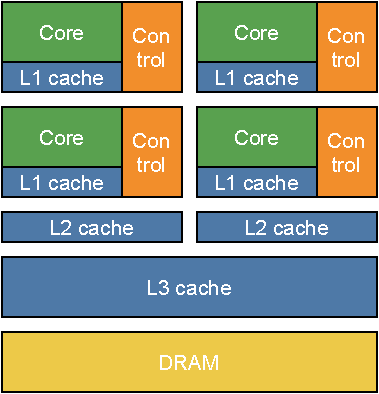
\includegraphics[width=\textwidth]{img/master_cpu_arch.pdf}
        \caption{Architecture of \acrshort*{acc:cpu}. Each core has L1 cache and own control circuit. Cores can therefore work independently.}
        \label{fig:cpuarch}
    \end{subfigure}
    \hfill
    \begin{subfigure}[t]{0.47\textwidth}
        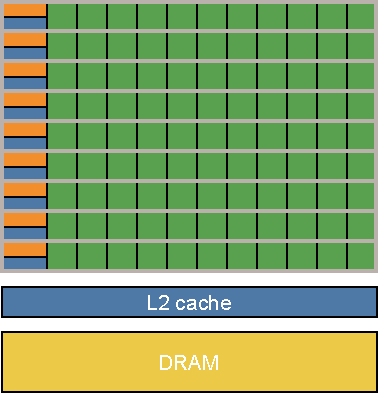
\includegraphics[width=\textwidth]{img/master_gpu_arch.pdf}
        \caption{Architecture of \acrshort*{acc:gpu}. One control circuit controls number of cores. One row of cores is called \acrlong{acc:sm} (\acrshort{acc:sm}, bounded by gray borders). L2 cache is shared between the cores.}
        \label{fig:gpuarch}
    \end{subfigure}
    \caption{Difference between \acrshort*{acc:cpu} and \acrshort*{acc:gpu} architecture}
\end{figure}

Computation power of \gpu comes from the fact, that it devotes in order of magnitudes more transistors on the chip to the data processing, rather than to the control circuits. The architecture of the \cpu is shown in figure \ref{fig:cpuarch}. Each core has its own control circuit and therefore each cores can execute instructions independently. Moreover, each thread has its own L1 cache.

The \gpu\index{GPU architecture} architecture is depicted in figure \ref{fig:gpuarch}. A set of cores share the same control circuit and L1 cache. One row of these cores is called \acrfull{acc:sm}. Number of cores per \acrshort{acc:sm} differ between architectures, more information can be found in the article by \citet{NVIDIAhistory} or on NVIDIA official websites. Using one control circuit to manage multiple cores brings some implications -- all the cores needs to execute the same instruction at once. In this sense, the instruction throughput is achieved using \acrfull{acc:simd} approach -- one instruction can at one tick modify multiple data. This is faster than executing the same instruction sequentially on \cpu.

Each \gpu come with different set of hardware features or available instructions. Compute capability\index{CUDA!compute capability} specify, which features are available at the target hardware. For example half--precision float--point operations are available from compute capability 5.3. Number of arithmetic CUDA cores per \acrshort{acc:sm} is 8 for compute capability 1.x, 32 resp. 48 for compute capability 2.0 resp. 2.1, 64 for compute capability 6.0, 7.x, and 8.0, 128 for compute capability 6.1, 6.2, and 8.6, and finally 192 for compute capability 3.x. I will therefore not discuss specific numbers in the following text. In order to use newer compute capabilities, the \gpu, driver and the software need to support them.

\acrlong{acc:cuda} allows almost direct translation of code from C onto the \gpu. It uses \cpp language with a few extensions. It is therefore straightforward to write program for \gpu as long as we are familiar with C syntax. To distinguish code running on \cpu and \gpu, \cuda differentiate between host (the code running on \cpu) and device (the code running on the \gpu) functions. There is special type of functions, called \emph{kernels}\index{CUDA!kernel}, that is called by the host, but executed on the device.

The \cuda defines following terminology:
\begin{itemize}
    \item CUDA thread\index{CUDA!thread} is execution of single kernel. To process $K$ blocks of data, the runtime creates at least $K$ threads and run the same kernel function on each of them.
    \item CUDA thread block\index{CUDA!block} is a set of threads grouped into grid. Programmer may specify size of the grid during call of the kernel function as a three--dimensional vector. The number of threads in the thread block is limited by the compute capability of the hardware. Moreover, all the threads in the thread block needs to be executed on one \acrshort{acc:sm} (with some exceptions) and can be synchronized using \textit{\_\_syncthreads} call. Each kernel receives \textit{threadIdx} variable, which allows to identify individuals threads in the block.
    \item CUDA kernel grid\index{CUDA!grid} is grid of thread blocks. Similarly to thread block, its size may be specified during  kernel call and each thread receives \textit{blockIdx} resp. \textit{blockDim} variables defining block in which the thread is running, resp. size of the blocks. More blocks from the same grid may run in parallel on different or same \acrshort{acc:sm}, but the threads cannot be synchronized between the blocks.
    \item Warp\index{CUDA!warp} is set of 32 threads (for all compute capabilities so far), that execute the same instruction. The thread block is split into warps and executed by the \acrshort{acc:sm}. The warp is the minimal unit executable on the \gpu. The device plan warps the same way \acrshort{acc:os} plans processes and may switch context to other warp while the current one is waiting for the data. By executing different warp, the latency of for example memory access is \enquote{hidden} behind execution of different warp. Although \gpu cannot execute anything smaller than warp, it may mask some threads from the execution. It is therefore possible to have block size of $50$ threads, however $2\cdot32 - 50=14$ cores in the second warp will still execute (although this fact is hidden from the programmer).
\end{itemize}

Because \cuda assumes a system composed of host and device, each of them have their own separate memory. Kernel are executing on the device and as such needs to have data its operating moved into the device memory as well. \cuda provides set of functions to allocate, deallocate, copy, and move memory between the host and the device\index{CUDA!memory management}. Similar to traditional \cpp programming, \cuda memory is allocated in a single unified linear address space. It can therefore reference each other using pointers and may use advanced data structures like linked lists and trees. Moving data between host and device is however time consuming, because the bandwidth between \cpu and \gpu is lower than memory transfers within the device memory. The copy memory from host to the device may generate nontrivial overhead, that may eliminate the advantage to use \gpu altogether, especially for small kernels. 

To minimize access latency to global device memory, \cuda provides a set of tools to speed up the process. It is possible to control L2 cache policy to better match executing kernels. It also provides functions to manage \emph{page--locked host memory}, which remains in the host memory and won't be paged by the \acrshort{acc:os}. Copying from this kind of memory can be done asynchronously, or when allocated as \emph{mapped--memory}, it is shared between the host and the device. Mapped--memory is implicitly transfer to and from the device and the programmer does not need to allocate it explicitly.

Special kind of memory, residing on--chip, is \emph{shared memory}\index{CUDA!shared memory}. The latency of shared memory is roughly 100x times lower than for global device memory and the global memory is shared in the thread block. Simple operation like matrix multiplication can be speed up by order of magnitude using shared memory \citep{MatrixMultiplicationGPU}. However, shared memory operates in equally--sized memory modules called banks, which complicates concurrent access to the shared memory. All the compute capabilities up today have 32 banks for shared memory organized into 32--bit words. Access to distinct memory addresses belonging to the same bank (bank conflict) by multiple threads within the same warp is serialized and therefore significantly increase the running time of the kernel. This is common for data types with the size of 64--bits, such as double precision floats. It may be beneficial to pad each value with one byte to eliminate conflicting access to the same banks.

As I mentioned earlier, all threads in the warp needs to execute the exact same instruction. However, the programming language supports conditional jumps, loops and other constructs known from the modern programming languages. It may easily happen, that some threads within the warp may execute different execution path -- situation known as \emph{warp divergence}\index{CUDA!warp divergence}. There are more reasons, why may threads in the warp diverge, but the branching is the most common one. In order for \gpu to evaluate each execution path, it runs them sequentially and mask out threads not participating in the current path. Masked threads will still execute the program, however, their results are ignored from the programmer point of view. This mean the same code will be executed twice (note that this increase exponentially for nested conditions) and significantly increase the time to finish the program. In general, warp divergence is undesirable and should be avoided when possible.
Warm divergence can only occur within a warp, different warps in the same thread block may execute different execution paths without any impact on the performance of the program.

Parallel nature of \cuda allows number of algorithms, that have by order of magnitudes better performance on \gpu than on \cpuns. Typical example would be element--wise linear operations or matrix multiplication \citep{GPUMatrixMultiplication}. Reduction operations such as summation of the array can be implemented effectively on \gpu \citep{harris2007optimizing}, as well as different kind of sorting algorithms \citep{GPUsorting}.

These operations are so common, NVIDIA released a set of libraries with implementation of these algorithms. The most relevant for this work are \textit{cuBLAS} (GPU--accelerated basic linear algebra library), CUDA Math Library implementing most common mathematical functions, and \textit{cuRAND} (GPU--accelerated random number generation). These implementations are optimized for the latest hardware and maintained by NVIDIA.




%%%%%%%%%%%%%%%
%%           %%
%%  PYTORCH  %%
%%           %%
%%%%%%%%%%%%%%%
\section{PyTorch}




%%%%%%%%%%%%%%%%%%%%%%%%%%%
%%                       %%
%%  EVA PARALLELIZATION  %%
%%                       %%
%%%%%%%%%%%%%%%%%%%%%%%%%%%
\section{Evolutionary Algorithms parallelization}
